\documentclass[14pt]{extarticle}
\usepackage{extsizes}
\usepackage{geometry}
\geometry{margin=0.5in}

%% for images
\usepackage{graphicx}
\graphicspath{ {images/} }

%% language support
\usepackage[T1,T2A]{fontenc}
\usepackage[utf8]{inputenc}
\usepackage[english,russian]{babel}

\usepackage{amsmath}
\usepackage{tikz}

%% hyperrefs
\usepackage{hyperref}
\hypersetup{
    colorlinks,
    citecolor=black,
    filecolor=black,
    linkcolor=black,
    urlcolor=black
}

\title{2024}
\author{КЫК}
\begin{document}
\maketitle
\tableofcontents

\section{Геометрическая оптика и её законы. Относительный и абсолютный показатель
преломления. Явление полного внутреннего отражения и его применение. Закон
обратимости световых лучей.}

\textbf{Четыре закона оптики:}
\begin{enumerate}
    \item Закон прямолинейного распространения света: 
    в однородной среде свет распространяется прямолинейно 
    \item Закон независимости световых лучей: 
    при пересечении световые лучи не возмущают друг друга
    \item Закон отражения света:
    отражённый луч лежит в одной плоскости с падающим лучом и 
    нормалью, восстановленной в точке падения. Угол падения равен 
    углу отражения. 
    \item Закон преломления света:
    преломленный луч лежит в одной плоскости с падающим лучом и нормалью,
    восстановленной в точке падения. Отношение синуса угла падения к синусу
    угла преломления есть величина постоянная для данных веществ:
    $\frac{\sin i_1}{\sin i_2} = n_{12} = const$
\end{enumerate}
Величина $n_{12}$ называется \textbf{относительным показателем преломления} 
второго вещества по отношению к первому.\\
Показатель преломления вещества по отношению к вакууму называется 
\textbf{абсолютным показателем преломления} данного вещества.\\\\
Предельный угол - такой угол падения, начиная с которого угол преломления 
равен $90^\circ$, т.е. свет не проникает во вторую среду и интенсивность
отраженного луча равна интенсивности падающего. Это явление называется
\textbf{полным внутренним отражением}.\\
Полное внутреннее отражение (т.е. отсутствие поглощения света) 
используется в волоконной оптике для передачи световых сигналов на большие
расстояния, а также в оптических приборах.\\\\
\textbf{Закон обратимости световых лучей:} если навстречу лучу, 
претерпевшему ряд отражений и преломлений, пустить другой луч, то 
он пойдет по тому же пути, что и первый (прямой) луч, но в 
обратном направлении. 

\section{Прохождение света через призму. Вывод угла отклонения при прохождении света
через призму с малым углом преломления}
Coming soon.
\section{Геометрическая оптика. Принцип Гюйгенса. Связь 
абсолютного показателя
преломления со скоростью распространения света в среде.}

\textbf{Принцип Гюйгенса:} каждая точка, до которой доходит
волновое движение, служит центром вторичных волн; огибающая
этих волн даёт положение фронта волны в следующий момент. 
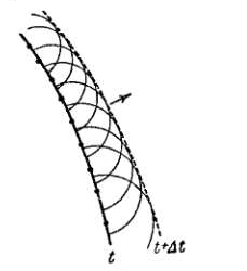
\includegraphics{wavefront.png}
Абсолютный показатель преломления $n$ и скорость распространения 
света в среде $v$ связаны соотношением: $n = \frac{c}{v}$, 
получаемым из волновой теории.
\\
\section{Световой поток. Кривая видности. Точечный источник.
Сила света и световой поток:
определения и единицы измерения}
\textbf{Световой поток} - поток лучистой энергии, оцениваемый
по зрительному ощущению. Полный световой поток равен 
$\Phi = \int_{0}^{\infty} V(\lambda) \phi(\lambda) d\lambda$,
где $V(\lambda)$ - функция видности, $\phi(\lambda)$ - 
функция распределения энергии потока по длинам волн, 
$\lambda$ - длина волны.\\
\textbf{Кривая видности} даёт чувствительность среднего нормального
человеческого глаза к излучению разной длины волны:
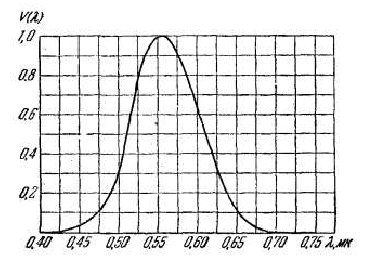
\includegraphics{visibility_curve.png} 
Как видно, максимум на длине волны 0.555 мк (зеленая часть спектра).
\\\\
\textbf{Точечный источник} - такой источник света, размерами
которого можно пренебречь по сравнению с расстоянием от места
наблюдения до источника.\\
\textbf{Сила света} - поток излучения точечного источника, 
приходящийся на единицу телесного угла: 
$I = \frac{d\Phi}{d\Omega}$. Единица измерения - свеча (св).\\
Единица измерения светового потока - люмен (лм).
1 лм = 1 св * 1 стер.
\section{Световой поток. Кривая видности. Освещенность, светимость, яркость: определения и
единицы измерения.}
\textbf{Освещенность} - характеризует степень освещенности 
поверхности падающим на неё световым потоком: 
$E = \frac{d\Phi_{пад}}{dS}$. Единица измерения освещенности - 
люкс (лк), 1лк = 1 лм : 1 м$^2$.\\
\textbf{Светимость} - световой поток, испускаемый единицей 
поверхности наружу по всем направлениям: 
$R = \frac{d\Phi_{исп}}{dS}$. Измеряется также в люксах. 
\section{Принцип Ферма. Оптическая длина пути. Вывод из принципа Ферма закона
отражения.}
\textbf{Принцип Ферма} - свет распространяется по такому пути,
для прохождения которого ему требуется минимальное время ИЛИ 
Свет распространяется по такому пути, оптическая длина которого 
минимальна.\\
\textbf{Оптическая длина пути} - величина 
$L = \int_{1}^{2} n ds$, где n - показатель преломления 
среды, $ds$ - длина элементарного отрезка пути.
\section{Принцип Ферма. Оптическая длина пути. Вывод из принципа Ферма закона
преломления.} 
Тут будут выводы.
\section{Геометрическая оптика. Основные понятия и определения: гомоцентрический и
астигматический пучок; стигматическое, действительное и мнимое изображение,
идеальная оптическая система, пространство предметов и пространство изображений.}
\textbf{Геометрическая (лучевая) оптика} - раздел оптики,
основывающийся на представлениях о световых лучах.\\
\textbf{Пучок} - совокупность лучей.\\
\textbf{Гомоцентрический пучок} - продолжения лучей 
пересекаются в одной точке. Ему соответствует сферическая
волновая поверхность. 
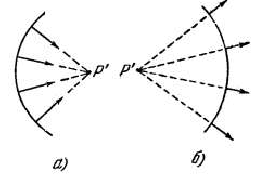
\includegraphics{beam_of_rays.png}
\textbf{Астигматический пучок} - пучок, которому соответствует
волновая поверхность двоякой кривизны. Лучи пересекаются
в совокупности точек, расположенных на двух взаимно перпендикулярных
отрезках.
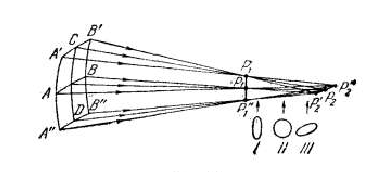
\includegraphics{beam_of_rays2.png}
Если оптическая система не нарушает гомоцентричности пучков,
то лучи, вышедшие из одной точки $P$, пересекутся также в одной
точке $P^{'}$ - \textbf{оптическом изображении} первой точки. Если 
любая точка предмета изображается в виде точки, то изображение
предмета называется \textbf{точечным (стигматическим)}.\\
Изображение \textbf{действительное}, если световые лучи 
действительно пересекаются в $P^{'}$, и \textbf{мнимое},
если в $P^{'}$ пересекаются продолжения лучей, проведенные
в направлении, обратном распространению света.\\
Оптическая система, дающая стигматическое изображение, 
геометрически подобное изображаемому предмету, называется
\textbf{идеальной}. С помощью такой системы 
пространственная непрерывность точек $P$ изображается 
в виде пространственной непрерывности точек $P^{'}$. 
Первая называется \textbf{пространством предметов}, вторая - 
\textbf{пространством изображений}.
\section{Центрированная оптическая система. Кардинальные точки и плоскости
центрированной оптической системы.}
Оптическая система, образованная сферическими (в частности
плоскими) поверхностями, называется \textbf{центрированной}, 
если центры всех поверхностей лежат на одной прямой. 
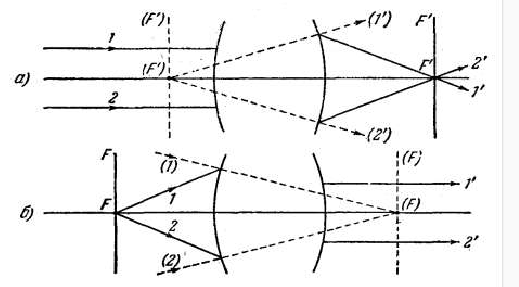
\includegraphics{optic_system.png}
\textbf{Кардинальные плоскости} - фокальные, главные и 
узловые плоскости.
\textbf{Кардинальные точки} - фокусы, главные точки и узлы.
\section{10. Центрированная оптическая система. Отражение и преломление на сферической
поверхности. Оптическая сила сферической поверхности.}
Похуй.
\section{Линза. Тонкая линза, её характерные точки и лучи. Оптическая сила. Построение
изображений в тонких линзах. Поперечное увеличение}
\textbf{Линза} - система двух сферических преломляющих 
поверхностей. 
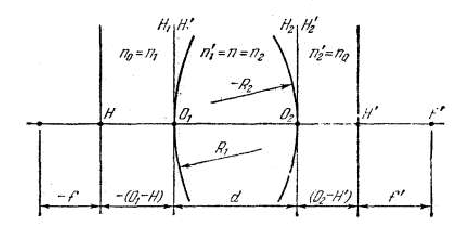
\includegraphics{lense.png}
Линза с пренебрежимо малым $d$ называется тонкой. В случае тонкой
линзы расстоянием $O_1 O_2$ можно пренебречь и считать их
находящимися в одной точке, называемой 
\textbf{оптическим центром} тонкой линзы. Любой луч, идущий
через него, не изменяет своего направления.\\
Оптическая сила тонкой линзы равна алгебраической сумме 
оптических сил преломляющих поверхностей:
$\Phi = \Phi_1 + \Phi_2$\\
\section{Вывод формулы тонкой линзы с использованием хода кардинальных параксиальных
лучей.}
\textbf{Формула тонкой линзы:} $\frac{1}{s^{'}} - 
\frac{1}{s} = \frac{n - n_0}{n_0} \bigl(\frac{1}{R_1}
-\frac{1}{R_2}\bigr)$
\section{Линза. Тонкая линза. Формула тонкой линзы. Аналитическое исследование формул
тонкой собирающей и рассеивающих линз}
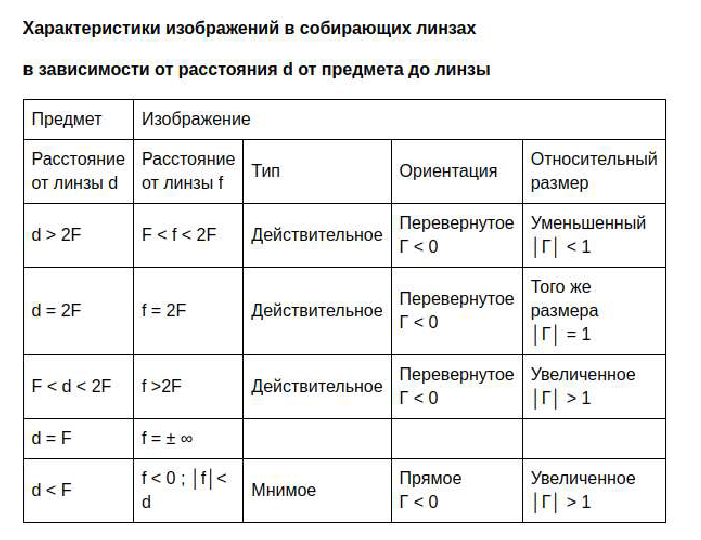
\includegraphics{lense_analysis.png}
\section{ Человеческий глаз как оптическая система (аккомодация, 
расстояния наилучшего зрения, дефекты зрения и их коррекция).}
\textbf{Аккомодация} - способность глаза менять фокусное расстояние
глаза посредством мышечного усилия, приспосабливаясь к 
расстоянию до рассматриваемого предмета. Ограничена снизу 20 см.\\
\textbf{Расстояние наилучшего зрения} - расстояние, на котором
нормальный глаз испытывает наименьшее напряжение при 
рассматривании деталей предмета.\\
\textbf{Близорукость} - дефект зрения, при отсутствии 
аккомодации изображение предмета лежит впереди сетчатки. 
Корректируется рассеивающей линзой.\\
\textbf{Дальнозоркость} - дефект зрения, при отсутствии 
аккомодации изображение предмета лежит за сетчаткой. 
Корректируется собирающей линзой.\\
\textbf{Астигматизм} - дефект зрения, искажённая кривизна 
роговицы и/или хрусталика, что провоцирует нечеткость изображения. 
Корректируется цилиндрическими линзами.\\
\section{Оптические приборы (лупа, микроскоп, зрительная труба). Увеличение прибора}
Bullshit.
\section{Световая волна. Уравнение световой волны в общем случае. 
Диапазон длин волн видимого света. Связь скорости распространения волны 
с (абсолютным) показателем преломления среды.}
\textbf{Световой вектор} - вектор напряжённости электрического поля.\\
\textbf{Уравнение световой волны} - закон, по которому изменяется
во времени и в пространстве проекция светового вектора: 
$A \cos (\omega t - kx + \alpha)$, $A$ - амплитуда световой волны.\\
Диапазон длин волн видимого света: 0.40-0.75 мк.\\
Скорость световой волны $v$ в среде с показателем преломления $n$ 
связана со скоростью волны $c$ в вакууме соотношением 
$v = \frac{c}{n}$.
\section{Световая волна. Уравнение световой волны. Интенсивность. Интерференция 
световых волн. Когерентные волны. Интерференционное слагаемое. 
Временная когерентность}
\textbf{Интенсивность света} $I$ в данной точке пространства - 
среднее по времени значение плотности светового потока, т.е. средний по 
времени световой поток через единицу поверхности площадки,
перпендикулярной к направлению распространения волны. $I \propto nA^2$\\
Пусть две волны одинаковой частоты, накладываясь друг на друга, возбуждают
в некоторой точке пространства колебания одинакового направления. 
Если разность фаз возбуждаемых волнами колебаний постоянна во времени, то
волны называются \textbf{когерентными}.\\
\textbf{Интерференция волн} - перераспределение 
светового потока в пространстве при 
наложении когерентных световых волн, в результате которого в одних местах 
возникают максимумы, а в других - минимумы интенсивности.\\
Интенсивность, наблюдаемая при наложении когерентных волн, задаётся формулой
$I = I_1 + I_2 + 2 \sqrt{I_1 I_2} \cos(\alpha_1 - \alpha_2)$. Третье слагаемое
называется \textbf{интерференционным}, т.к. именно оно задаёт распределение
интенсивности в пространстве. 
\textbf{Временная когерентность} - неизменность разности фаз двух колебаний 
с течением времени в данной точке пространства.\\
\section{Интерференция световых волн. Оптическая разность хода (с выводом). 
Условие интерференционного максимума и минимума}
\textbf{Оптическая разность хода} -  величина, равная разности оптических
длин проходимых волнами путей: $\Delta = L_2 - L_1$.\\
Условие интерференционного максимума: $\Delta = \pm k\lambda_0 \
(k = 0, 1, 2, ...)$ (целое число длин волн)\\ 
Условие интерференционного минимума: $\Delta = \pm \bigl(k+\frac{1}{2}\bigr)
\lambda_0 \ (k = 0, 1, 2, ...)$ (полуцелое число длин волн)
\section{Интерференция световых волн. Опыт Юнга, интерференционная картина от двух
точечных источников (с выводом)}
Похуй. 
\section{Интерференция световых волн. Опыт Юнга, интерференционная картина от двух
точечных источников (без вывода). Координаты максимумов и минимумов
интерференции (с выводом). Ширина интерференционной полосы}
Координаты максимумов интенсивности: 
$x_{max} = \pm k \frac{l}{d} \lambda_0 \ (k = 0, 1, 2, ...)$\\
Координаты минимумов интенсивности: 
$x_{min} = \pm \bigl(k+\frac{1}{2}\bigr) \frac{l}{d} \lambda_0 
\ (k = 0, 1, 2, ...)$\\
\textbf{Ширина интерференционной полосы} $\Delta x$ - расстояние между 
двумя соседними минимумами интенсивности.
\section{Интерференция света. Способы наблюдения интерференции света. Метод Юнга.}
Источником света служит ярко освещённая щель, от которой свет падает на две
узкие равноудалённые щели. Таким образом, световая волна разделяется на две. 
Интерференция света наблюдается на экране, там, где световые волны 
накладываются друг на друга. На экране наблюдаются чередующиеся тёмные 
и светлые полосы. 
\section{Интерференция света. Способы наблюдения интерференции света. Зеркала Френеля
(вывод ширины полосы и числа полос).}
\section{Интерференция света. Способы наблюдения интерференции света. Бипризма Френеля
(вывод ширины полосы и числа полос)}
\section{Интерференция световых волн. Интерференция при отражении от тонких плёнок.
Условие наблюдение максимума интенсивности (с выводом).}
При падении световой волны на тонкую прозрачную пластинку или плёнку 
происходит отражение от обеих поверхностей пластинки. В результате возникают
когерентные световые волны, которые могут интерферировать.\\
Условие максимума интенсивности: 
$2b \sqrt{n^2 - \sin^2 i_1} = \bigl(k + \frac{1}{2}\bigr) \lambda_0$, где
$b$ - толщина пластинки, $k$ - порядок интерференционного максимума. 
\section{Интерференция световых волн. Кольца Ньютона. Радиусы светлых и темных колец
Ньютона (с выводом).}
Кольца Ньютона - полосы равной толщины. Наблюдаются при отражении света 
от соприкасающихся друг с другом плоскопараллельной стеклянной пластинки 
и плосковыпуклой линзы с большим радиусом кривизны. Роль тонкой плёнки 
играет воздушный зазор между пластинкой и линзой. 
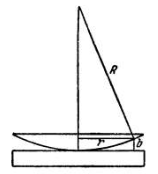
\includegraphics{newton_rings.png}
Радиусы колец Ньютона: $r = \sqrt{\frac{R \lambda_0}{2} (m-1)} \ 
(m = 1, 2, 3, ...)$. Чётные m - светлые кольца, нечётные - тёмные. 
$m = 1$ - точка касания пластинки и линзы. 
\section{Применение интерференции света. Интерферометрия.}
Интерференция используется для определения показателей преломления газов, 
для высокоточного измерения длин и углов и т.д. Приборы, в которых применяется
интерференция, называются интерферометрами. 
\section{Дифракция света. Принцип Гюйгенса-Френеля. 
Определения дифракции Френеля и дифракции Фраунгофера}
Дифракция - совокупность явлений, наблюдаемых при распространении света в среде
с резкими неоднородностями и связанных с отклонениями от законов геометрической
оптики. Она наиболее сильно выражена при длинах волн, сравнимых с размерами
препятствий.\\
Если источник света и точка наблюдения $P$ расположены от препятствия настолько 
далеко, что лучи, падающие на препятствие и лучи, идущие в точку $P$, 
образуют параллельные пучки, говорят о 
\textbf{дифракции Фраунгофера (дифракции в параллельных лучах)}. В противном 
случае говорят о \textbf{дифракции Френеля}. 
\section{Дифракция света. Принцип Гюйгенса-Френеля. Зоны Френеля, радиус внешней
границы зоны Френеля (с выводом).}
Найдём амплитуду светового колебания, возбуждаемого в точке $P$ сферической
волной, распространяющейся в однородной среде из точечного источника $S$.
Волновая поверхность такой волны симметрична относительно прямой $SP$. Тогда 
можно разбить её на кольцевые зоны так, чтоб расстояния от краёв каждой зоны 
до точки P отличались на $\frac{\lambda}{2}$. 
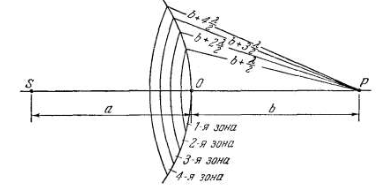
\includegraphics{frenel_zones.png}
Радиус внешней границы $m$-й зоны равен $r_m = \sqrt{\frac{ab}{a+b}m \lambda}$,
$a$ - радиус волновой поверхности,  
$b$ - расстояние от вершины волновой поверхности $O$ до точки $P$.
\section{Дифракция света. Принцип Гюйгенса-Френеля. Зоны Френеля, радиус внешней
границы зоны Френеля (без вывода). Амплитуда результирующего колебания (без
вывода).}
Амплитуда, создаваемая в некоторой точке $P$ сферической волновой 
поверхностью, равна половине амплитуды, создаваемой центральной зоной:
$A = \frac{A_1}{2}$. Т.е. действие всей волновой поверхности эквивалентно 
половине действия центральной зоны. 
\section{Дифракция света. Дифракция Френеля от круглого отверстия – дифракционная
картина (с пояснениями).}
\section{Дифракция света. Дифракция Френеля от круглого диска – дифракционная картина (с
пояснениями). Пятно Пуассона}
\section{Дифракция Фраунгофера. Дифракция от щели. Условие минимумов. Дифракционная
картина от щели}
Условие минимумов: $b \sin \phi = \pm k \lambda \ (k = 1, 2, 3, ...)$
\section{Дифракция света. Дифракционная решетка. Период решетки. Условие главных
максимумов. Порядок главного максимума. Дифракционная картина от решетки.}
\textbf{Дифракционная решётка} - совокупность большого числа одинаковых,
отстоящих друг от друга на одно и то же расстояние щелей.\\
\textbf{Период (постоянная) решётки} - расстояние $d$ между серединами соседних
щелей.\\
Условие главных максимумов: $d \sin \phi = \pm m \lambda 
(m = 0, 1, 2, ...)$. $m$ называется \textbf{порядком главного максимума}.
Максимум нулевого порядка 1, далее их по два.\\
Дифракционная картина от решётки:
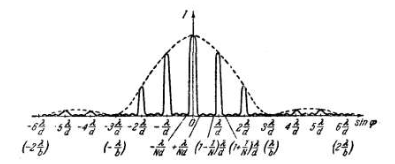
\includegraphics{difraction_pattern.png}
\section{Дифракционная решётка как спектральный прибор. Угловая дисперсия. Линейная
дисперсия. Разрешающая способность.}
Положение главных максимумов зависит от длины волны. Поэтому при пропускании
через решётку белого света все максимумы, кроме центрального, 
разложатся в спектр, фиолетовый конец которого обращён к центру дифракционной 
картины, красный - наружу. Таким образом, дифракционная решетка может быть 
использована как спектральный прибор.\\
Основными характеристиками спектрального прибора являются его дисперсия и 
разрешающая сила.\\
Угловая дисперсия: $D = \frac{\delta \phi}{\delta \lambda}$, где
$@d \phi$ - угловое расстояние между спектральными линиями, отличающимися 
по длине волны на $@d \lambda$. Для дифракционной решётки 
$D \approx \frac{m}{d}$.\\
Линейная дисперсия: $D_{лин} = \frac{\delta l}{\delta \lambda}$, где 
$\delta l$ - линейное расстояние на экране или на фотопластинке между
спектральными линиями, отличающимися по длине волны на $\delta \lambda$. Для
дифракционной решётки $D_{лин} = f^{'} \frac{m}{d}$, где $f^{'}$ - 
фокусное расстояние линзы, собирающей дифрагирующие лучи на экране.\\
Разрешение спектральных линий - их раздельное восприятие. Разрешающая сила 
спектрального прибора - безразмерная величина 
$R = \frac{\lambda}{\delta \lambda}$. Для дифракционной решётки $R = mN$, где
$m$ - порядок спектра, $N$ - число щелей. 
\end{document}
